\paragraph{Sơ đồ tuần tự luồng tải lên tài liệu cá nhân}

Luồng nghiệp vụ này mô tả
quá trình người dùng tải lên tài liệu cá nhân.
Document Service kiểm tra subscription, validate file, lưu metadata, upload file gốc lên Cloudflare R2
và gửi task xử lý nền qua Celery (RabbitMQ).

\begin{table}[H]
\centering
\renewcommand{\arraystretch}{1.3}

\begin{tabular}{|l|l|p{5cm}|}
\hline
\textbf{Thành phần} & \textbf{Phân loại} & \textbf{Vai trò trong hệ thống} \\ \hline
User & Actor & Người dùng tải lên tài liệu cá nhân. \\ \hline
Web Frontend & Component & Giao diện web Next.js. \\ \hline
API Gateway (Kong) & Component & Cổng API chuyển tiếp các yêu cầu API. \\ \hline
Document Service & Microservice & Kiểm tra quyền, validate file, lưu metadata và xuất bản công việc xử lý nền. \\ \hline
Document Database & Database & Lưu tài liệu và gói thuê bao người dùng. \\ \hline
Cloudflare R2 & Object Storage & Lưu file gốc của người dùng. \\ \hline
RabbitMQ & Message Broker & Nhận Celery task. \\ \hline
\end{tabular}
\caption{Các thành phần tham gia luồng tải lên tài liệu cá nhân}
\end{table}

\begin{figure}[H]
\centering
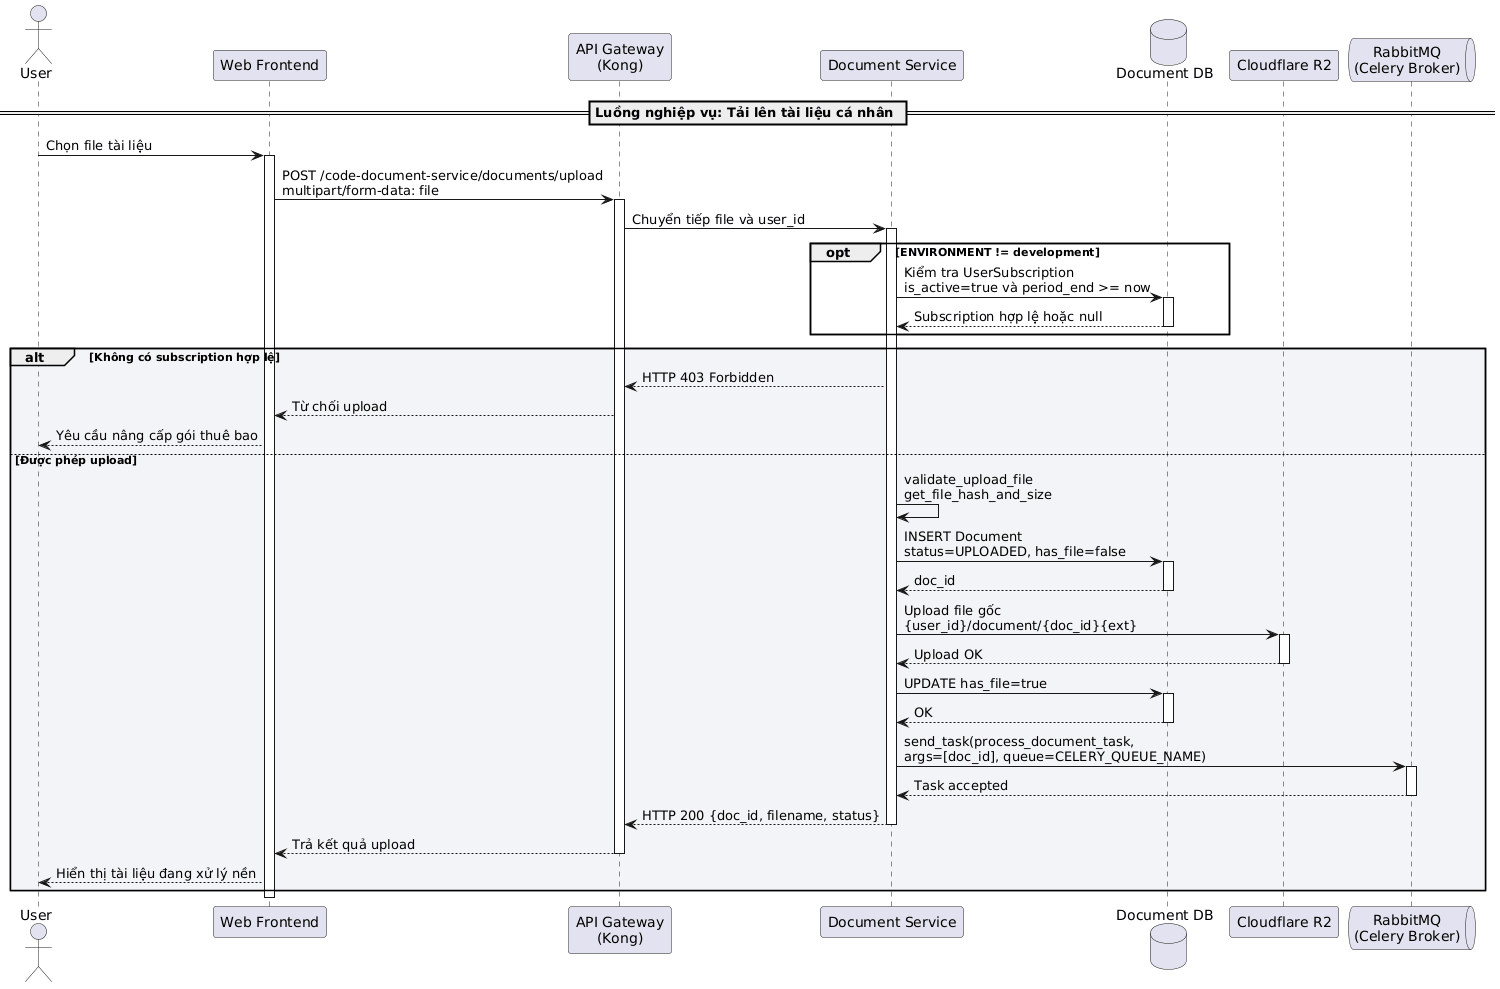
\includegraphics[width=0.95\textwidth]{contents/Sequence/UML-Sequence-UserUploadPersonalDocument.png}
\caption{Sơ đồ tuần tự luồng tải lên tài liệu cá nhân}
\end{figure}

\subparagraph{Mô tả tổng quan}

\begin{itemize}

\item \textbf{Yêu cầu tải lên:}
Người dùng chọn tải lên tài liệu cá nhân.
Giao diện gửi yêu cầu tải lên tệp tin qua
cổng API tới dịch vụ quản lý tài liệu.

\item \textbf{Kiểm tra gói thuê bao:}
Dịch vụ tài liệu
kiểm tra trạng thái hoạt động
và thời hạn của gói thuê bao VIP
của người dùng trong hệ thống.

\item \textbf{Tạo bản ghi tài liệu:}
Tệp tin được kiểm tra tính hợp lệ,
tính toán mã băm kiểm tra,
kích thước tệp và
tạo bản ghi tài liệu mới
trong CSDL tài liệu.

\item \textbf{Tải tệp lên kho chứa:}
Tệp tài liệu gốc
được tải lên kho lưu trữ trực tuyến
dưới thư mục riêng của người dùng
và cập nhật trạng thái
tài liệu đã có tệp tin.

\item \textbf{Đăng ký công việc nền:}
Dịch vụ gửi một công việc xử lý tài liệu
vào hàng đợi công việc
để thực hiện phân tích tài liệu trong nền.
\end{itemize}
